\documentclass[11pt,a4paper]{article}
  	\usepackage[pdftex]{graphicx}
	\usepackage{times}
	\usepackage[simplified]{pgf-umlcd}

\setlength{\parindent}{0mm}
\setlength{\oddsidemargin}{-5mm}
\setlength{\evensidemargin}{-5mm}
\setlength{\textwidth}{165mm}
\setlength{\textheight}{250mm}
\setlength{\topmargin}{-10mm}
\setlength{\marginparwidth}{15mm}
\setlength{\marginparsep}{7mm}

\begin{document}

\title{\textbf{Complex Class UML Design}}
\author{Last Updated: Iain Bertram}
\date{22 February 2019}
\maketitle


\begin{center}
\begin{tikzpicture}
	\begin{class}[text width=10cm]{Complex}{0,0}
	\attribute{- realpart: double}
	\attribute{- imagpart : double}
	
	\operation{$\ll$constructor$\gg$ Complex() }
	\operation{$\ll$constructor$\gg$ Complex(x: double, y: double) }
	\operation{+ setComplex(x: double, y: double): void}
	\operation{+ getReal(): double}
    \operation{+ getImag(): double}
       \operation{+ increaseBy(z: Complex): void}
    \operation{+ conjugate(): void}
    \operation{+ print(): void}
    \operation{+   add(z: Complex, w: Complex) Complex $\ll$static$\gg$}
	\end{class}

\end{tikzpicture}
\end{center}


In addition to the class diagram we need a complete description of the
class as well, including tests to check that the class is working as
it should. For the example Complex class we could write:

{\bf Complex} is a class representing complex numbers given by ($a +
bi$) where $a$ and $b$ are stored in two doubles \texttt{realpart} and
\texttt{imagpart}.

{\bf \underline{Constructors}:}\\
{\bf Complex():} is the default constructor where \texttt{realpart=0} and
\texttt{imagpart=0}. \\
{\it Check that the object of type complex is created and its components are set to zero.}

{\bf Complex(x: double, y: double):} is a constructor where
\texttt{realpart=x} and \texttt{imagpart=y}. \\
{\it Check that the complex is created and its components are set to $x$ and $y$ for the cases $x=1, y=1$ and $x=0, y=1$ and $x=-1, y=1$ and $x=-1, y=0$}


{\bf \underline{Methods}:}

{\bf +setComplex(x: double, y: double): void}: sets the complex number
so that \texttt{realpart=x} and \texttt{imagpart=y}. \\
{\it Create a complex number $5+3i$ and set it to be $-4+5i$ and check
  that it is changed correctly.}

{\bf +getReal(): double}: return \texttt{realpart}

{\bf +getImag(): double}: return \texttt{imagpart}

{\bf +increaseBy(z: Complex): void}: Let $z=a+bi$ and c=\texttt{realpart}
and d=\texttt{imagpart} then the method will modify the complex number such that
\texttt{realpart}$=c+a$ and \texttt{imagpart}$=d+b$.
{\it Check this with $1+1i$ and $z=0$, $z=1$, $z=i$, $z=1-1i$, $z=-1+1i$}

{\bf +add(z: Complex, w: Complex): Complex}: return  $(a+c)+(b+d)i$ where $z=a+bi$ and $w=c+di$. (\emph Static Method)\\
{\it Check this with $z=1+1i$ and $w=0$, $w=1$, $w=i$, $w=1-1i$, $w=-1+1i$}

{\bf +conjugate(): void}: sets \texttt{imagpart}$=-$\texttt{imagpart}.\\
{\it Check this by setting the complex number equal to several different values including zero and $i$ and checking that the complex number has been correctly set to be the complex conjugate.}

{\bf +print(): void}: print the Complex number with the format $a+bi$
to standard output.\\
{\it Set the complex number to several different values including zero and check that the
  output is correct.}

Note: The tests that we have constructed should attempt to cover all possible
kinds of occurrences with the class. I.e. we need to check standard and
non-standard cases such as the complex number being zero or purely real or purely
imaginary.

\end{document}
